\section{$Re_{\tau}=2000$ simulation} 
The last simulation performed is carried out at $Re_{\tau}=2000$, which in terms of channel width and bulk velocity is equivalent to $Re_{b}=...$.\par
The bulk velocity is 19.79, $\alpha_{0}$ is 0.5 and $\beta_{0}$ is equal to 1.\par
The timestep is constant, with \emph{dt}=... and the simulation time is T=5. \par
Once again the excessive resource requests lead us to reduce the simulation time to just few non-dimensional units, however, in order to guarantee good results, we sampled the field every 0.05 steps, so that we can employ a 100 fields to do the ensemble average.\\~\par
The grid employed in this simulation face 1000 points in the wall-normal direction, 4096 in the spanwise direction and 4096 points along the streamwise dimension. The mesh size is extremely huge, with more than 8 billions of points.\par
We reported a summary of the simulation configuration in table~\ref{table:2000}\\~\par

\begin{table}
\caption{Simulation data for $Re_{\tau}$=2000}
\begin{center}
\begin{tabular}{ccccccccccccc}
\toprule
$L_{x}$ & $L_{z}$ & $\delta$ & $nx$ & $nz$ & $ny$ & $\alpha_{0}$ & $\beta_{0}$ & $\Delta x^{+}$ & $\Delta z^{+}$ & $px$ & $dt$ & $T$\\
$4\pi$ & $2\pi$ & 1 & 4096 & 4096 & 1000 & 0.5 & 1 & tbd  & tbd & 1 & tbd & 5 \\
\bottomrule
\end{tabular}
\end{center}
\label{table:2000}
\end{table}


The disk space requirement raised approximately by a factor of 10, with 400GB of disk space needed per each field. This reason pushed us once again to rely in live post processing, instead of saving snapshots of the field.\\~\par

The statistics gained from the simulation are here presented.\par
We start from figure~\ref{loglaw:2000}, which report the law of the wall. The data seems to fit better than previous simulations the theoretical behavior, characterized by $k=0.41$ and $B=5.2$.
Consequently towards the centerline the velocity defect law seems to approximate our results very precisely, as shown by the graph~\ref{velocity:defect:2000}.\\~\par

\begin{figure}
\begin{center}
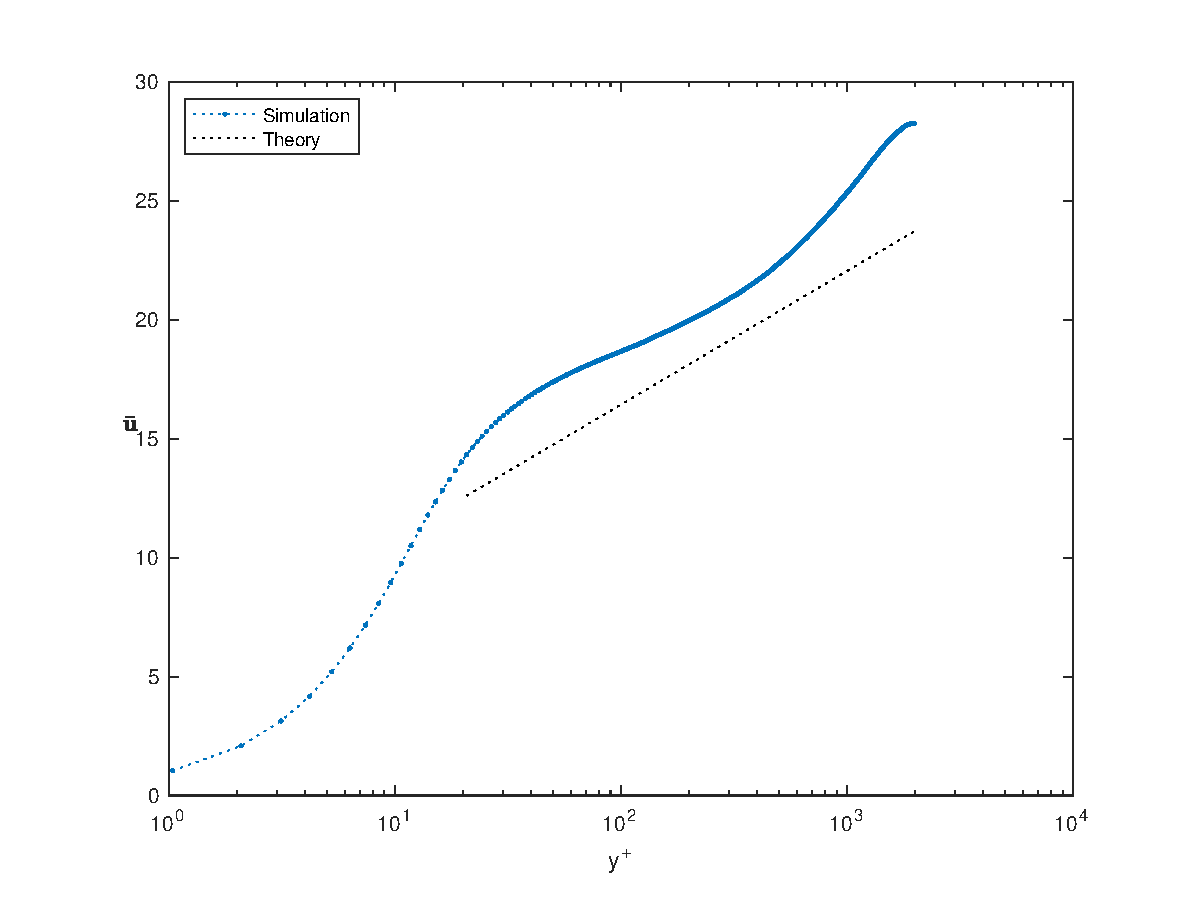
\includegraphics[scale=0.55]{grafici/loglaw_2000.eps}
\caption{$\bar{u}^{+}$ in the near wall region for a $Re_{\tau}=2000$ simulation}
\label{loglaw:2000}
\end{center} 
\end{figure}

\begin{figure}
\begin{center}
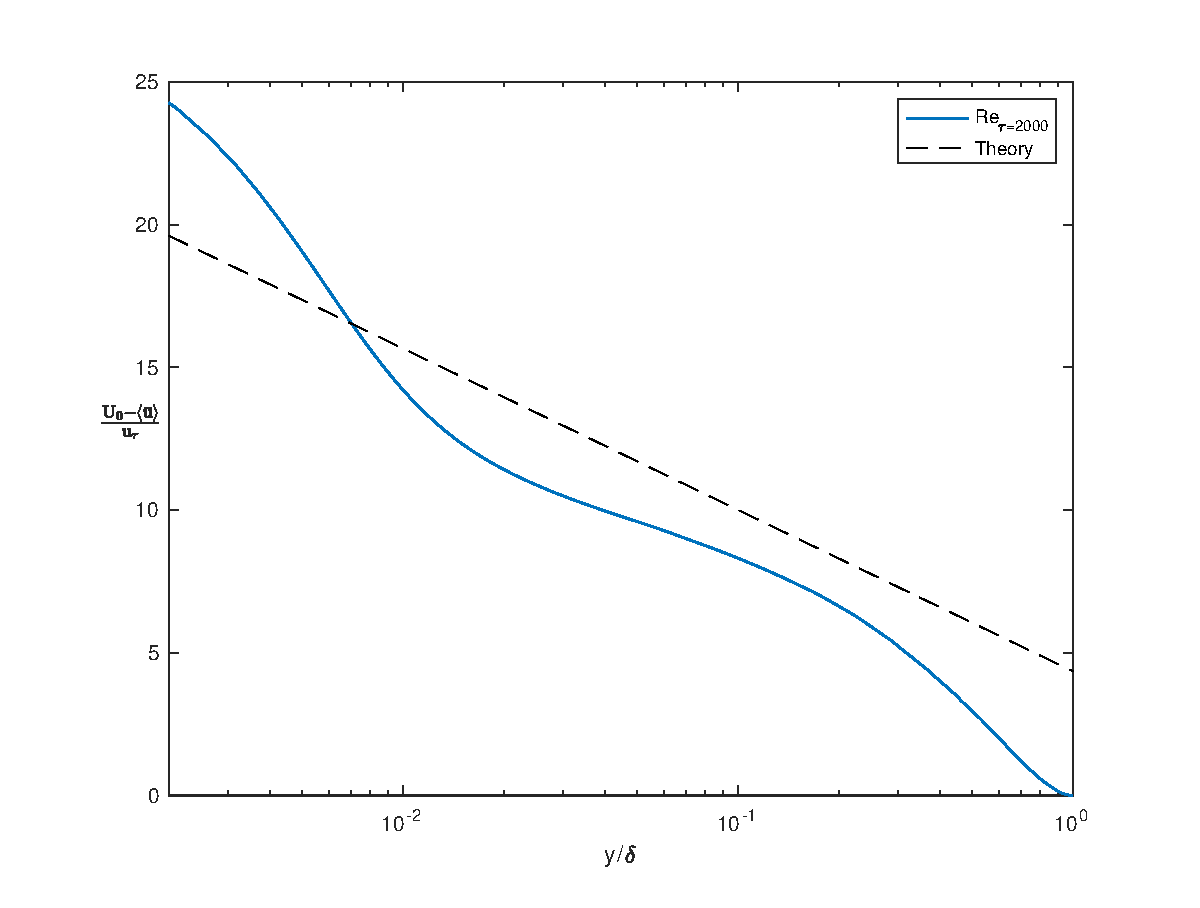
\includegraphics[scale=0.55]{grafici/velocity_defect_2000.eps}
\caption{Velocity defect for a $Re_{\tau}=2000$ simulation}
\label{velocity:defect:2000}
\end{center} 
\end{figure}

In figure~\ref{budget:2000} we reported the \emph{rms} fluctuations, normalized by the $u_{\tau}^{2}$, jointed with the TKE distribution. The first difference we can see by comparing this graph with the others is related to the peak values, which have incremented again, in line with our expectations for a more turbulent flow. \par
This time we can see that, followed by the raise in peak values, the spanwise and streamwise fluctuations exhibit a wider basement, with more energy   associated to those distances from the wall. This fact is partially due to the reduced lengthscale of this simulation with respect to the previous.\par
However, as the lens magnify, despite of the higher $Re_{\tau}$, the turbulence still tend to exhibit itself as a bi-dimensional phenomena close to the wall, exactly what happens also for \emph{low Reynolds} simulations.\par

Reaching the centerline the \emph{rms} terms and the TKE curve tends to aligne with the values of the $Re_{\tau}=1000$ simulation.\\~\par

\begin{figure}
\begin{center}
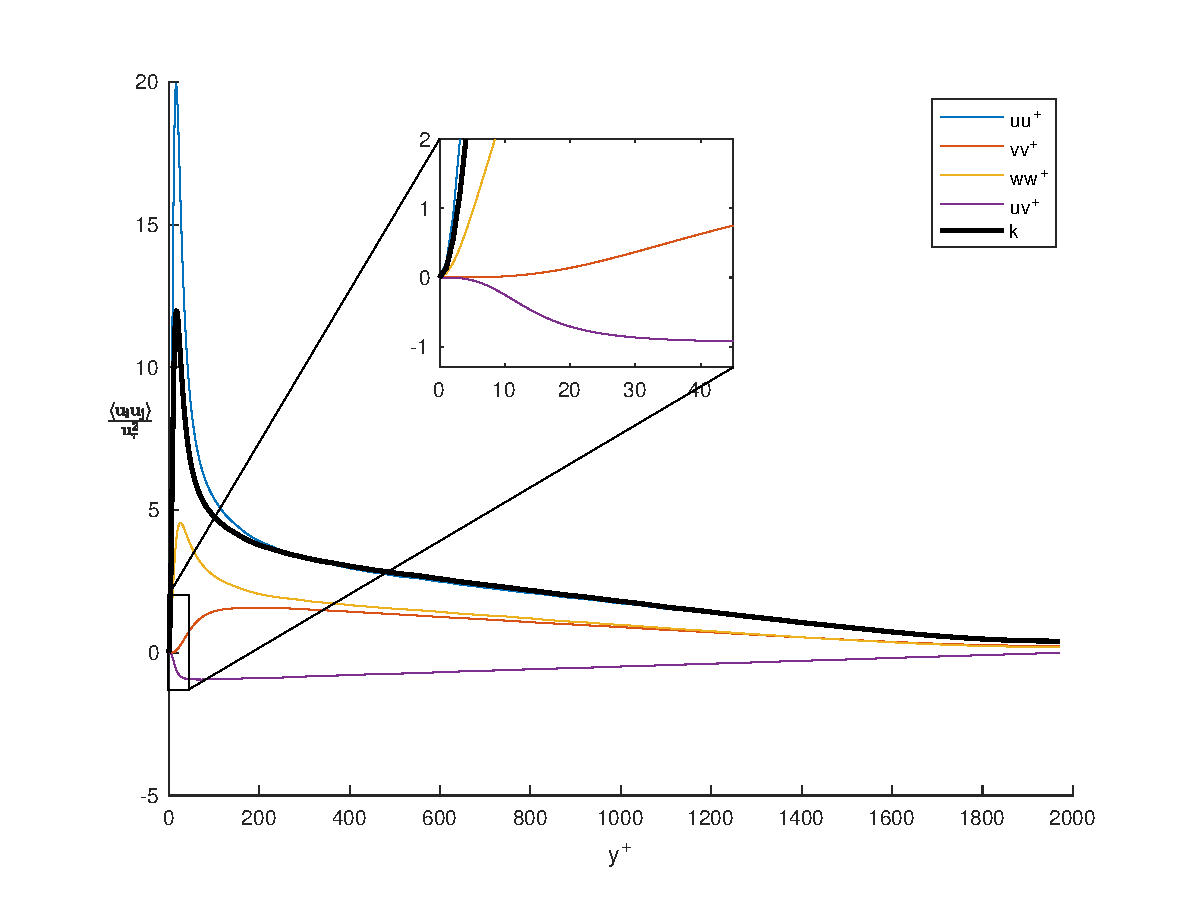
\includegraphics[scale=0.55]{grafici/budget+k_2000.eps}
\caption{\emph{rms} terms for a $Re_{\tau}=2000$ simulation}
\label{budget:2000}
\end{center} 
\end{figure}


The finer mesh and the higher Reynolds evidenced the appearance of a new turbulence peak, detached from the wall-cycle, identified by knees in the curves represented in figure~\ref{rms:1000}. Although the profiles are similar, with exception for the higher peaks reached, in the near wall region, they behave differently moving towards the inner region of the flow. In particular, by looking at $u'/u_{\tau}$, the sketchy knee present around $y^{+}\approx 100$ in figure~\ref{rms:kmm:180} now results to be fully developed and has moved towards the centerline, approximately around $y^{+}\approx 400$. The peak does not differ too much in the two simulations, with values of $2.6\sim2.7$ located at $y^{+}\approx14$, however, the higher energy content manifest through the trailing values. These terms shows an upward bias, if compared with the $Re_{\tau}=180$ values, plus the presence of the already cited knee.\par
Similar behavior is expressed by $w'/u_{\tau}$, although in its case the increase in terms of peak value is consistent, with a slightly decrease of the peak coordinate towards $y^{+}\approx30$. Also in this case the appearance of the knee is approximately around $y\approx 400$.\par
Also the term $v'/u_{\tau}$ face a huge increment of the peak value, in first approximation we may say that it doubles its value with respect to $Re_{\tau}=180$ simulation. In such case identifying the knee is less straightforward. However, we can observe that the area under the curve has clearly increased.\\~\par

\begin{figure}
\begin{center}
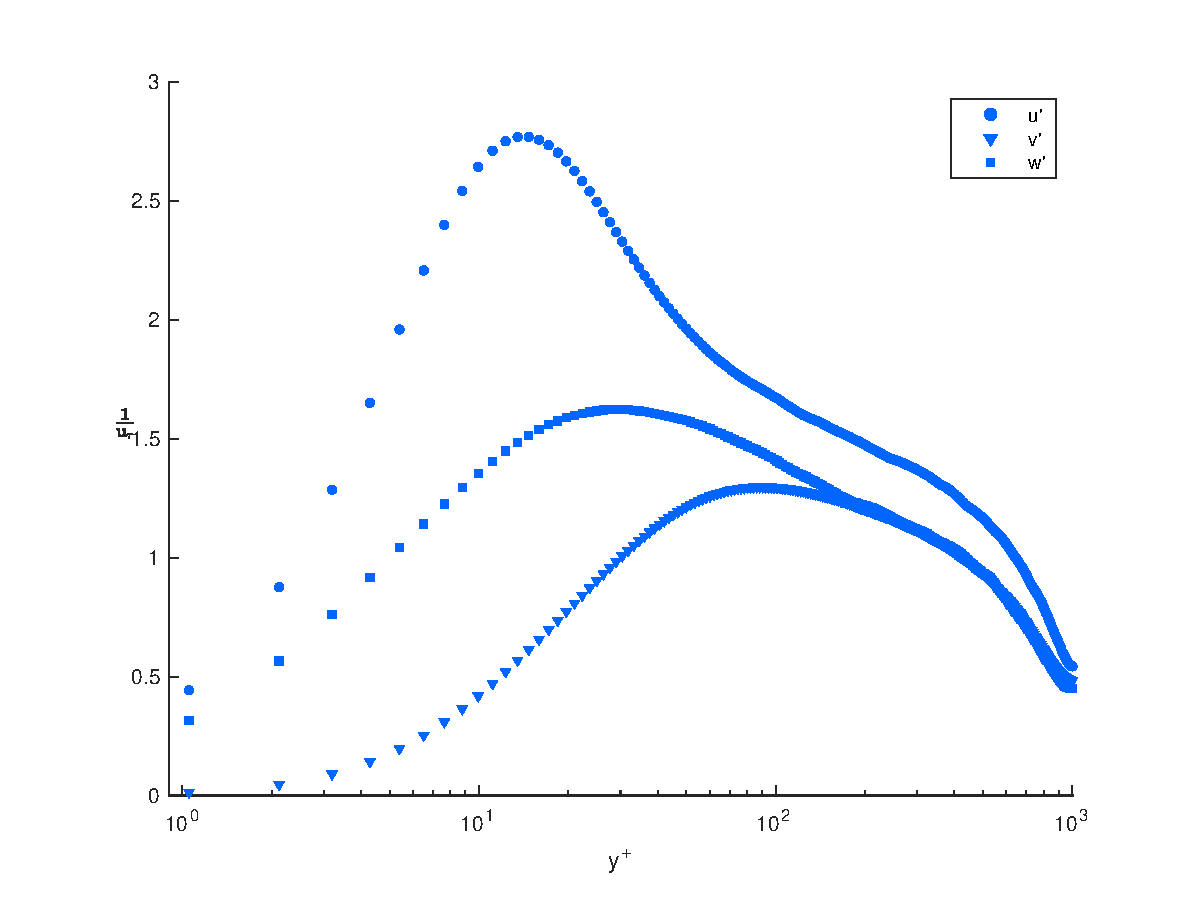
\includegraphics[scale=0.55]{grafici/rms_1000.eps}
\caption{\emph{rms} behavior on a $Re_{\tau}=1000$ simulation}
\label{rms:1000}
\end{center} 
\end{figure}

\begin{figure}
\begin{center}
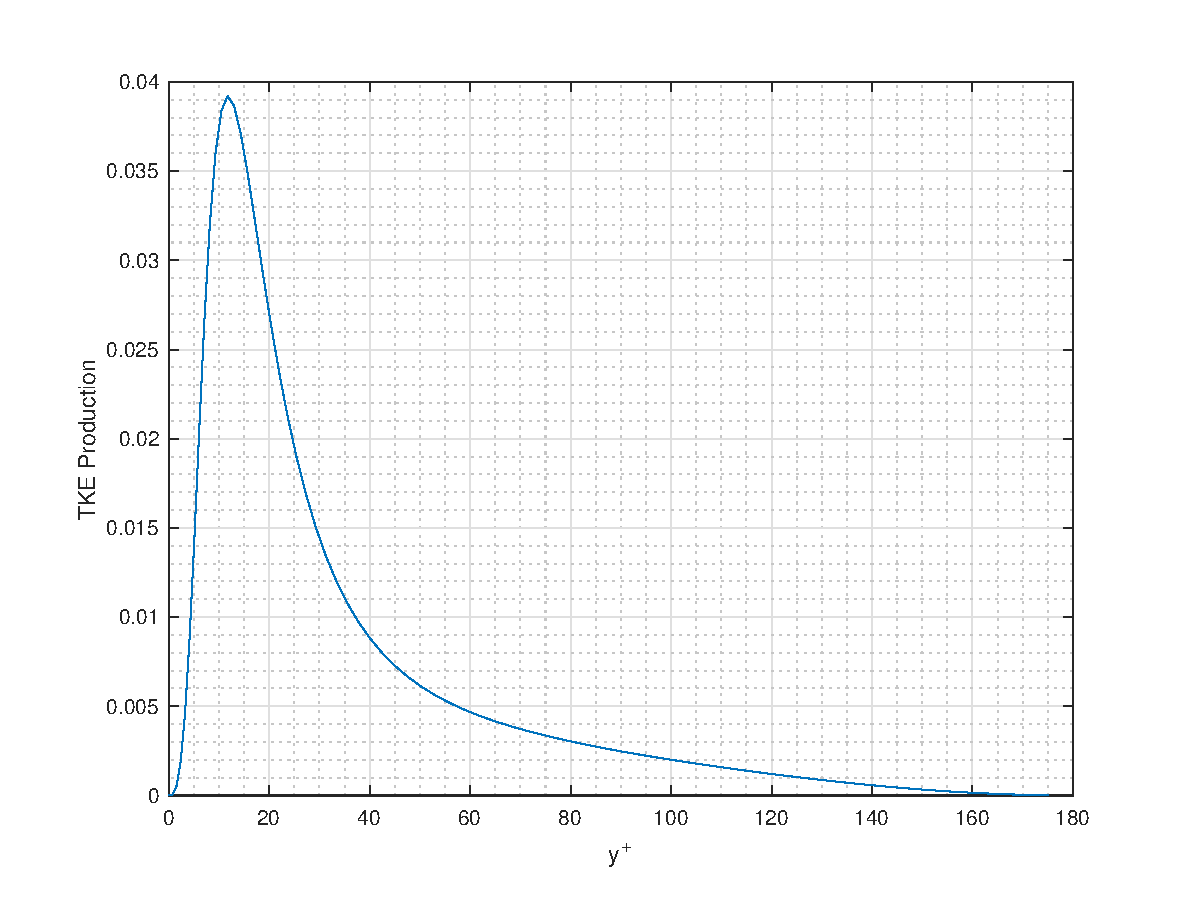
\includegraphics[scale=0.55]{grafici/tke_prod_1000.eps}
\caption{Production term of the TKE eq. for a $Re_{\tau}=1000$ simulation}
\label{tke:prod:1000}
\end{center} 
\end{figure}

An upward shift is expressed also by the \emph{rms} terms near the wall. Nevertheless the curves does not exhibit marked changes in shape with respect to its counterpart in the previous simulation, as figure~\ref{wall:rms:1000} testify, with the streamwise and spanwise components that depart from zero as $y^{+}$, while the wall-normal components leave the wall as $y^{2+}$. \\~\par

Similar reasoning applies also for the graphs of the \emph{production}, reported in figure~\ref{tke:prod:1000}, that reach a slightly higher peak of $P/Re_{\tau}=0.24$, without showing significant changes of the curve shapes. The peak is still located nearby $y\approx 12$.\\~\par

As theory affirms, the wall coordinate of the peak of production corresponds to that in which the stress components become equivalent. This aspect will be detailed further, comparing the results of all the simulations together.
At the present we limit to present the behavior of the stress components, which is reported in figure~\ref{stresses:1000}.

\begin{figure}
\begin{center}
\includegraphics[scale=0.55]{grafici/wall_rms_1000.eps}
\caption{Normalized \emph{rms} close to the wall for a $Re_{\tau}=1000$ simulation}
\label{wall:rms:1000}
\end{center} 
\end{figure}

\begin{figure}
\begin{center}
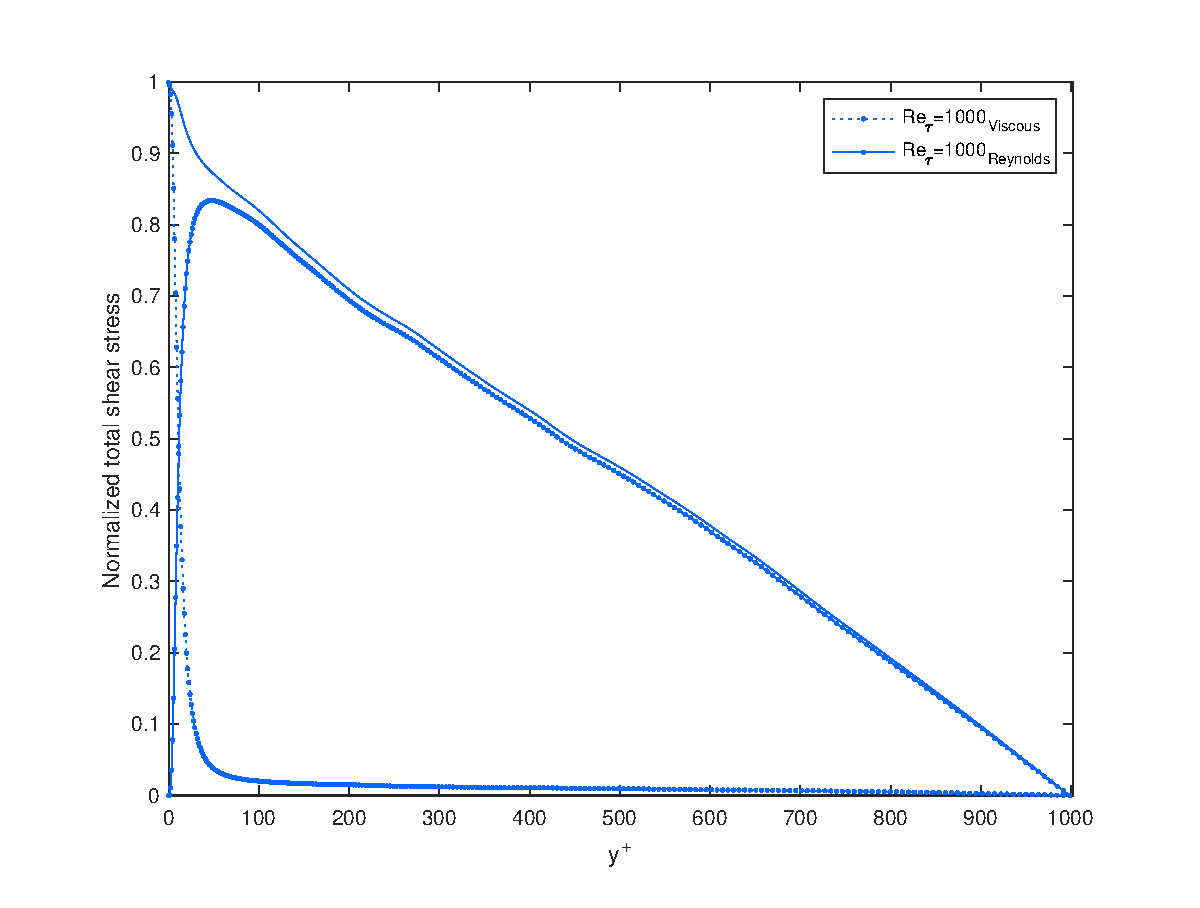
\includegraphics[scale=0.55]{grafici/stresses_1000.eps}
\caption{Normalized total shear stress for a $Re_{\tau}=1000$ simulation}
\label{stresses:1000}
\end{center} 
\end{figure}